% \section{\mc スペクトログラムを画像とみなした手法(提案手法1)}
% \subsubsection{\mc 最大エントロピー法によるスペクトル密度推定}
% スペクトログラムの獲得には最大エントロピー法を用いる。
% フーリエ変換を用いたスペクトル密度推定法にはEEGには成り立たないであろう
% 仮定を要請しなければならないが、最大エントロピー法はウィーナー・ヒンチンの定理以外の一切の仮定を必要としないため、
% ロバストな推定が可能である。
% 最大エントロピー法のスペクトル密度推定法を時間窓をずらしながらEEGに適用することでスペクトログラムを獲得する。

% \subsubsection{\mc 画像認識の手法の適用}
% Convolution層は通常画像認識のために用いられるが、スペクトログラムからERDを検知する研究は従来より盛んであり、
% これは人間がERDを可視化、画像化してきたことに他ならない。
% スペクトログラムをERDの生じる周波数を特定するために用いるのではなく、
% 直接、畳み込みニューラルネットワークに与えることで分類させることを試みた。


\section{\rm FilterBank Network \mc(提案手法1)}
\subsubsection{\rm Convlution\mc 層によるFIR フィルタバンク}
EEGを\(X\in \mathbb R^{M\times N\times 1}\)とする。
ここに、\(M\)は電極の数、\(N\)はサンプル点数、\(1\)は後に周波数を示すためのダミーインデックスである。
\(X\)に対するConvolution層による演算は以下で表される。
\begin{equation}
    u_{m,n,k} = \sum_{c=1}^C\sum_{p=0}^{P-1}\sum_{q=0}^{Q-1} x_{m+p,n+q,c} h_{p,q,c,k} + b_{m,n,k}
\end{equation} 
この演算に関して、\(P=1,b_{m,n,k}=0,C=1\)でパラメータを与えることにより、
\begin{equation}
    u_{m,n,k} = \sum_{q=0}^{Q-1} x_{m,n+q,1} h_{1,q,1,k}
    \label{eq:pseudoFIR}
\end{equation} 
という演算を行うことができる。
ここでパラメータ\(H\in \mathbb R^{1\times D\times 1\times K}\)と与えることで、
フィルタ次数\(Q-1\)のFIRフィルタ\(K\)個からなるフィルタバンクとなる。

\subsubsection{\rm Convlution\mc 層による空間フィルタ}
続いて、第2層について\(Q=1\)でパラメータを与えることにより
\begin{equation}
    v_{m,n,l} = \sum_{p=0}^{P-1} u_{m+p,n,k} g_{1,q,1,k}
    \label{eq:pseudoFIR}
\end{equation} 
という演算を行うことが可能であり、EEGに対して電極の重み付けを行っていることに相当する。
ここで\(g\)がパラメータである。

以降ニューラルネットワークの演算を適宜定義することで、
2層目以降の層は、EEGを入力としたフィルタバンクからの出力を受け取ることが可能となる。
本研究では2層目以降もConvlution層のみを用いて特徴量の抽出を試みた。
提案手法におけるデータの形状の変化について図\ref{fig:pseudFBCSP}に示す。
\begin{figure}[t]
    \centering
    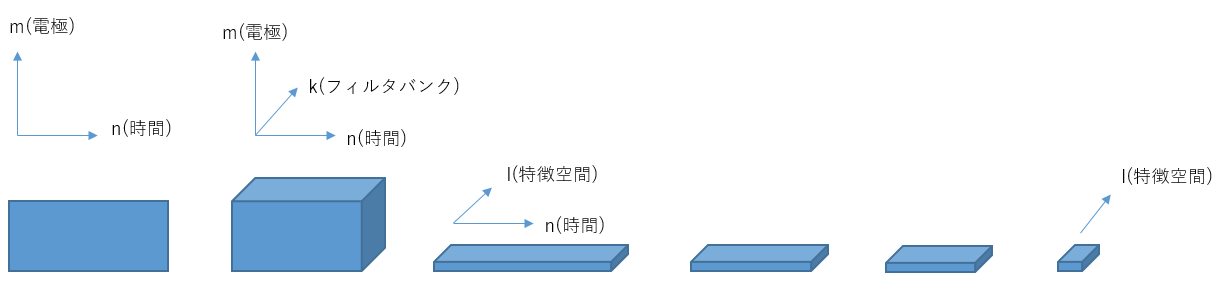
\includegraphics[width=13cm]{images/pseudFBCSP.png}
    \caption{Convlution層を用いたFIRフィルタバンクによるデータの形状変化}
    \label{fig:pseudFBCSP}
\end{figure}

同時に最適化可能な点である。具体的なニューラルネットワークの構造は実験結果と共に記す。


\section{\rm 3DConvlution + 2DConvLSTM\mc (提案手法2)}
\subsubsection{\mc 高階テンソルとしての \rm EEG\mc データ構造}
通常、EEGのデータは時間の次元を持つサンプル点数と空間的な情報を有する電極をインデックスとした
2階テンソルとして表現されるが、本論文では運動想起時のEEGは時間、電極、周波数をインデックスとした
高階テンソルで表されると仮定する。
この仮定はEEG従来より周波数帯域毎に異なる脳波として捉えられてきたこと、
特定の身体部位に対応する脳の領域が局所的であること、時系列データであることから妥当であると考えられる。

また電極のインデックスについては任意の配置によってテンソル化がなされるが、
頭皮上の空間的配置によって電極間の関連性は異なっている。
したがって時間、電極、周波数のインデックスに関して
電極のインデックスの取り方を2次元に展開し
時間、頭皮上の座標1、頭皮上の座標2、周波数をインデックスとする4階テンソルとして捉え直す。

この場合におけるEEGの測定データは
EEGが\(X\in \mathbb R^{M_1\times M_2\times N\times 1}\)と与えられ、
Convlution層を用いたFIRフィルタバンクは、3DConvlution層を用いることで以下の式で書き換えられる。
\begin{eqnarray}
    u_{m_1,m_2,n,k}& = &\sum_{c=1}^C\sum_{p_1=0}^{P_1-1}\sum_{p_2=0}^{P_2-1}\sum_{q=0}^{Q-1} x_{m_1+p_1,m_2+p_2,n+q,c} h_{p_1,p_2,q,c,k} + b_{m_1,m_2,n,k}\\
    u_{m_1,m_2,n,k}& = &\sum_{q=0}^{Q-1} x_{m_1,m_2,n+q,1} h_{1,1,q,1,k}
    \label{eq:pseudoFIR3D}
\end{eqnarray} 
\(u_{m_1,m_2,n,k}\)について\(m_1,m_2\)が頭皮上の座標を表すインデックスである。
3DConvlutionによるデータの形状の変化を図\ref{fig:pseudFBCSP3d}に示す。


\subsubsection{\rm ConvLSTM}
ConvLSTMは、通常のLSTMのLinear層の計算をConvolution層に変更することで
入力\(X = (X_1,\cdots,X_T)\in \mathbb R^{M_1 \times M_2 \times T \times K}\)を受け取り
出力\(Y = (Y_1,\cdots,Y_T)\in \mathbb R^{M_1' \times M_2' \times T \times C}\)を出力する。
ここに\(C\)は任意の正数であり、\(M_1',M_2'\)はパラメータの与え方で決定される。
この構造を入れることによって、
電極のインデックスを頭皮上に展開しフィルタバンクを通過した4階テンソルEEGを入力として受け取ることができる。
ここでConvLSTM内でのCovolution演算は頭皮上の2次元に対して行い、LSTMの処理は時間方向に行うようにする(図\ref{fig:ConvLSTM})。

この手法には頭皮空間上でEEGを観測しながら、
その時間経過を追うことで運動想起部位を分類するというモデルを構築する狙いがある。
また、頭皮上に展開された2次元に対してConvolution演算を用いることは、
電極配置が距離的に近い場合において強い関連性を有するという仮定が入る。
Convolutionの演算時にパラメータのサイズによって覆われる空間的領域以外の部分は
全く関連しないという無限に強い事前分布を与えることになるためである。
しかし実際にはConvolution層を積層することによって、空間的に離れた電極間にも
関連性を有する形に修正が可能であるため、事前分布を与えながらも、
実際の関連性の探索はニューラルネットワークの学習によって獲得される。
\begin{figure}[t]
    \centering
    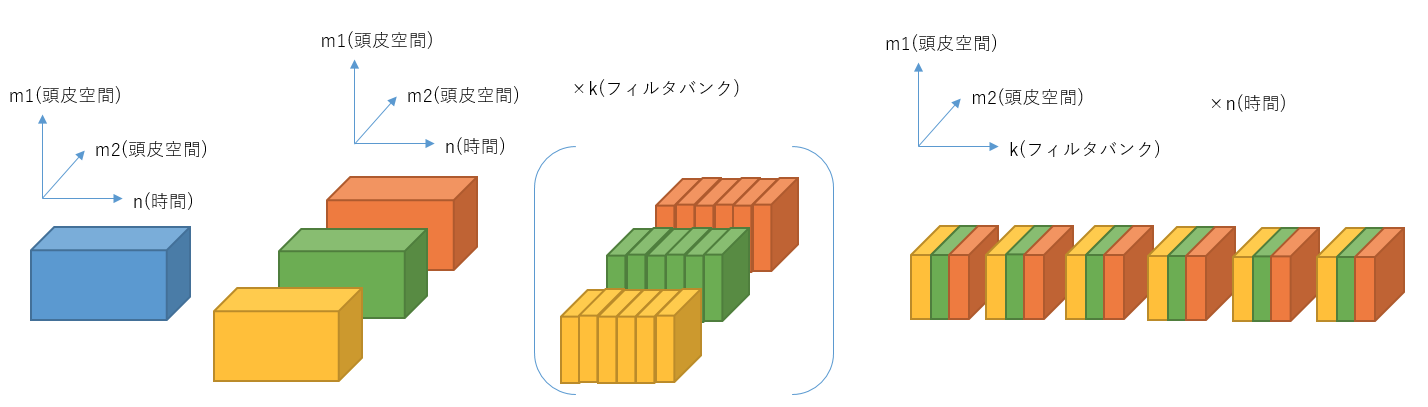
\includegraphics[width=13cm]{images/pseudFBCSP3d.png}
    \caption{3DConvlution層を用いたFIRフィルタバンクによるデータの形状変化}
    \label{fig:pseudFBCSP3d}
\end{figure}
\begin{figure}[t]
    \centering
    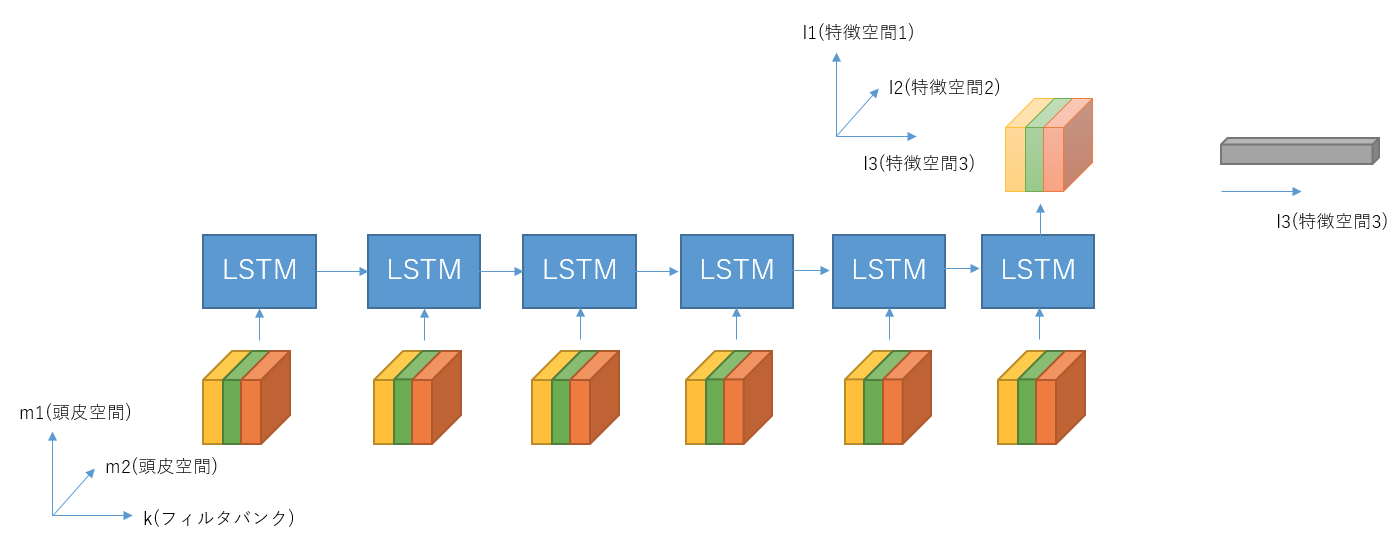
\includegraphics[width=13cm]{images/ConvLSTM2d.png}
    \caption{ConvLSTMによるデータ形状変化}
    \label{fig:ConvLSTM}
\end{figure}

このような仮定を置くことの妥当性を示すものとして、
信号源推定を行う際にグラフフーリエ領域へ変換を行うことで
良い推定結果が得られるという東らの研究\cite{グラフフーリエ}がある。
グラフフーリエでも、空間的に距離の近い電極によって測定されるEEGほど
類似性が高いという仮定が決定論的に与えられる。
